\documentclass{article}
\usepackage{amsmath} % For mathematical formulas
\usepackage{graphicx} % For including images
\usepackage{xcolor} % For the Kouci brand palette
\usepackage{tikz}
\usepackage{fontspec}
\usepackage{tabularx}
\usepackage{booktabs}
\usepackage[table]{xcolor}
\usepackage{array}
\usepackage{float}

% Center text horizontally and vertically
\newcolumntype{C}[1]{>{\centering\arraybackslash}m{#1}}
\newcolumntype{Y}{>{\centering\arraybackslash}X}

% Custom colors
\definecolor{headerblue}{HTML}{17365D}
\definecolor{lightblue}{HTML}{EDF3F8}


\definecolor{KouciGreen900}{HTML}{1B2114}
\definecolor{KouciGreen800}{HTML}{303B24}
\definecolor{KouciGreen700}{HTML}{465536}
\definecolor{KouciGreen600}{HTML}{5C7047}
\definecolor{KouciGreen500}{HTML}{738A59}
\definecolor{KouciGreen400}{HTML}{8FA475}
\definecolor{KouciGreen300}{HTML}{B2C0A2}
\definecolor{KouciGreen200}{HTML}{D9E0D1}

\setmainfont{Fira Sans}


\title{Kouci Threat Model}
\author{Pedro Camargo}
\date{November 2026}



\begin{document}

\thispagestyle{empty}
\setmainfont{Fira Sans}

\makeatletter
\AddToHookNext{shipout/background}{%
\begin{tikzpicture}[remember picture,overlay]
    \node[inner sep=0pt] at (current page.center) {%
        
\includegraphics[width=\paperwidth,height=\paperheight]{imgs/cover-water.png}%
    };
    \fill[KouciGreen900,opacity=0.50]
        (current page.south west) rectangle (current page.north east);

\end{tikzpicture}%
}

\AddToHookNext{shipout/foreground}{%
\begin{tikzpicture}[remember picture,overlay]
    \node[inner sep=0pt]
        at ([xshift=-2.5cm,yshift=-1.65cm]current page.north east) {%
            
\includegraphics[height=3cm]{imgs/kouci-logo.png}%
        };
    

    \node[anchor=west,text width=0.72\paperwidth,align=left,text=white]
        at ([xshift=2.05cm,yshift=1.2cm]current page.west) {%
            {\sffamily\bfseries\fontsize{38}{43}\selectfont
             Kouci Threat Model}\par
            \vspace{0.25cm}
            {\color{KouciGreen400}\rule{10cm}{2.2pt}}\par
            \vspace{0.45cm}
            {\large\color{KouciGreen200}
             Security and privacy analysis for an
             offline-first water polo analytics platform}
        };

    \node[anchor=center,text width=0.72\paperwidth,align=center,text=white]
        at ([yshift=1.2cm]current page.south) {%
            {\large\color{KouciGreen200}
            \today}
        };

    
\end{tikzpicture}%
}
\makeatother

\null
\clearpage


\setcounter{page}{1}

\tableofcontents
\newpage

\section{Executive Summary}

This document defines the threat model for a controlled Android testbed that reproduces two security-sensitive flows from Kouci:

\begin{enumerate}
    \item A paid-feature licensing flow
    \item Local storage and processing of a synthetic scouting dataset
\end{enumerate}



This model uses \textbf{STRIDE per Element} analysis, complemented by \textbf{STRIDE per Interaction} analysis at the key trust boundaries. It identifies threats in six categories and relates them to assets, data flows, adversary capabilities, defensive controls and validation evidence.

The study investigates observed attack effort against defined objectives and defender costs of \textbf{three} separate protections: R8, local APK signing-certificate verification, and Android Keystore-backed data encryption.

The attacker has a copy of the application and controls its execution device. The exact privileges and instrumentation capabilities are recorded per attempt.

The same researcher develops the variants and performs the attacks (Pedro Camargo). Consequently, any observed differences are specific to the analyst, variants, order and conditions tested, and cannot by themselves establish the causal effect of a control on a general attacker population.

The two attack objectives, three variants, separate pilot, frozen protocol, measured outcomes and limitations are specified in the dissertation proposal. The threat identifiers, boundary names, tables, diagrams and document structure below are organisational choices introduced for this threat-model draft, not claims that the experimental design has been finally approved.

This document has two layers of purpose:

\begin{enumerate}
    \item \textbf{Dissertation experimental core:} license bypass (G1) and unauthorized recovery of an entire fixed synthetic scouting dataset (G2), independently evaluating R8, local signing-certificate verification and Android Keystore-backed encryption.
    \item \textbf{Kouci product security:} complementary risks concerning synchronization/backend, accounts, availability, statistics integrity, backups and distribution. These are architectural hypotheses or potential extensions, not verified components or minimum experimental objectives.
\end{enumerate}

\subsection{About Kouci Project}

Kouci is a water polo analytics application for coaches, teams and analysts. It records matches and opponent scouting data and includes paid features according to the user's license. It follows an \textbf{offline-first} approach, part of the application logic, data, and license verification must reside on the device, without continuous communication with a trusted server. There's only one call to the server for license verification, which is done at the first launch of the application (onboarding).

Kouci's foundation is built on the principles of security and privacy by design, since the world of sports analytics is highly competitive and sensitive, with a lot of attackers trying to steal data and gain unfair advantages with piracy. This document presents the threat model of the Kouci application, which is a crucial step in understanding the security and privacy risks associated with the application.

Below is a quick overview of the architecture of the application, which is relevant for understanding the threat model.

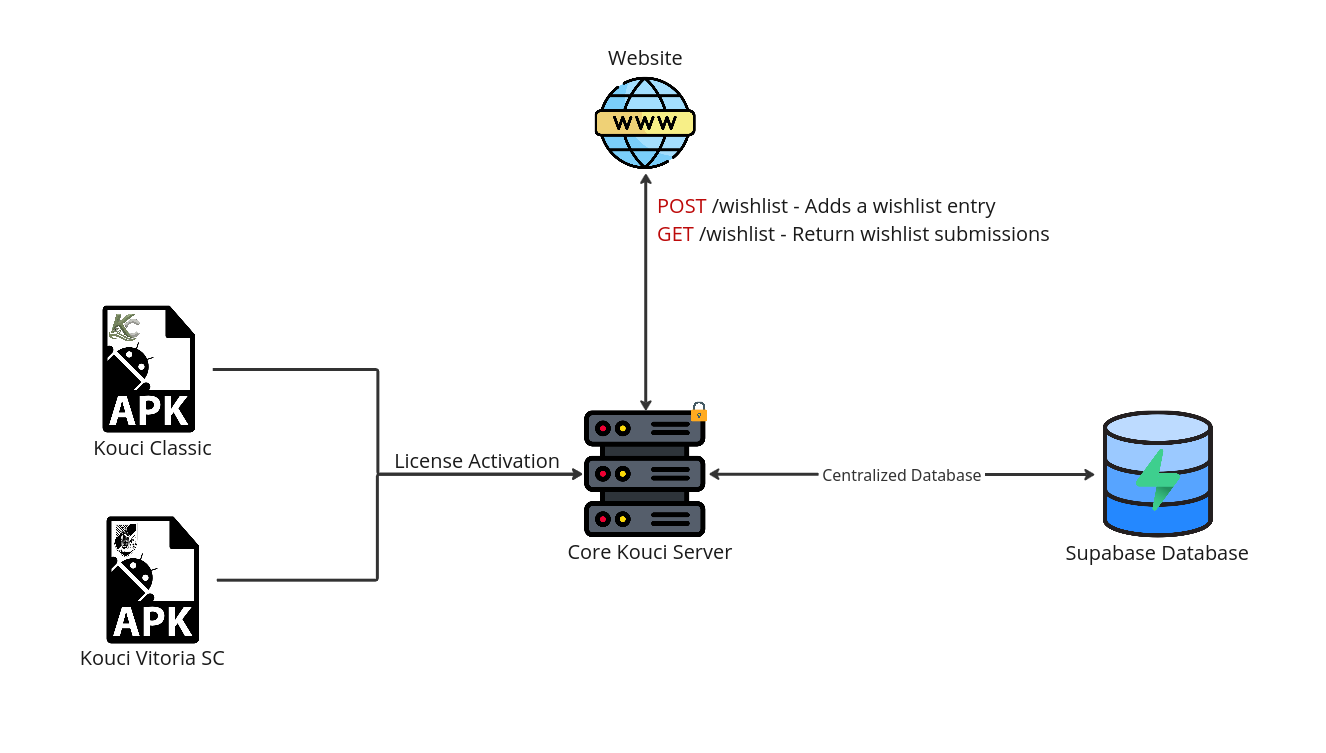
\includegraphics[width=\linewidth]{imgs/Architecture.png}

Kouci is a mobile application that runs on Android devices. It is built using the React Native with Expo framework, which allows for cross-platform development. The application uses a local SQLite database to store data, and it communicates with a backend server for license verification and data synchronization.

A publicly accessible web application currently allows prospective users to join a wishlist ahead of Kouci's official launch. Although this web application is part of the broader Kouci ecosystem, it falls outside the scope of this threat model. Its existence is acknowledged solely to provide context about the ecosystem and does not introduce additional components, attack surfaces, or trust boundaries into the security analysis.

\subsection{Kouci Future Work}

In the future, there will be more features, such as a web app for coaches and analysts to view and analyze data, a backend server for data synchronization and storage, custom builds for different teams and leagues built in the cloud, championships and tournaments tracking, live match tracking, game analysis with machine learning, and more. These features will introduce new security and privacy risks that will need to be addressed in future threat models.

\section{Methodology}

\subsection{Questions to answer}

\subsubsection{What are we protecting?}

Licensed features, authorization logic, complete scouting data, signing identity, cryptographic material and traceable experimental evidence. The most important asset is the mobile application itself, which is the target of reverse engineering and tampering attacks, the source of income and the foundation of the entire Kouci ecosystem. 

\subsubsection{What can go wrong?}

Our main application can be reverse engineered, modified and redistributed by an attacker. The attacker can bypass licensing checks, access sensitive data of other teams, and compromise the integrity of the application. This can lead to financial loss, reputational damage, and potential legal issues for Kouci.

\subsubsection{What are we doing about it?}

Mitigate and monitor the risks through a combination of technical controls and continuous monitoring. This includes implementing code obfuscation, secure storage of sensitive data, detection of tampering attempts, and regular security assessments.

It's important to note that securing an application against \textbf{Reverse Engineering} completely is impossible, but by implementing these measures, we can significantly reduce the risk of successful attacks and protect the assets of Kouci.

\subsubsection{Did we do a good enough job?}

To know all the objectives are met, we need to perform a series of tests and evaluations. Use observable experiments, reproducible success criteria, explicit preconditions, step logs and results.

\subsection{In scope for the dissertation}

What we firstly must focus is having a controlled testbed to evaluate the effectiveness of the three protections (R8, local signing-certificate verification and Android Keystore-backed encryption) against two attack objectives. It must be an unprotected baseline APK with the syntetic dataset stored in plaintext. 

First we should target to execute a specified paid feature \textbf{without a valid license} (G1) and then \textbf{recover the entire synthetic scouting dataset outside the normal user interface}. The dissertation will focus on these two objectives, which are the most critical for the security of the application.

While developing and testing the protections, an observation of the attack effort, defender costs, integration complexity, APK size and performance impact will be made. This will provide a comprehensive understanding of the effectiveness of the protections and their impact on the overall user experience.

\subsection{Exclusions and Assumptions}

The minimum study excludes comprehensive production hardening, attacks against a real backend, continuous online validation, the distribution/build pipeline, real user data, desktop evaluation, isolated hardware-backed versus software-backed key comparisons, remote attestation and additional anti-instrumentation mechanisms. Such areas appear only as complementary risks.

Root access, an unlocked bootloader, instrumentation, the ability to read other applications' private files and operating-system compromise are not assumed. They are scenario-specific preconditions, not universal attacker capabilities.

\newpage

\section{Assets}

\subsection{Primary Assets}

These are assets that provide direct value to the business and are the main targets of attacks.  

\renewcommand{\arraystretch}{1.8}
\begin{table}[htbp]

\small
\begin{tabularx}{\textwidth}{
    C{0.5cm}
    C{3cm}
    Y
}

\rowcolor{KouciGreen700}

\multicolumn{1}{c}{\color{white}\textbf{ID}} &
\multicolumn{1}{c}{\color{white}\textbf{Asset}} &
\multicolumn{1}{c}{\color{white}\textbf{Description}} \\

A1 &
Player Personal Data &
Names, birth years, cap numbers, positions and associated player information. \\

\hline

A2 &
Match Statistics &
Shots, saves, exclusions, penalties, assists, turnovers, and individual performances. \\

\hline

A3 &
Team Tactical Information &
Tactical analysis, opponent weaknesses, shot patterns, and strategic information. \\

\hline

A4 &
Company Reputation &
Customer trust, product credibility, and confidence in the platform's security. \\

\hline

A5 &
Customer Data &
Information associated with clubs, coaches, subscriptions, and customer relationships. \\

\hline

A6 &
Software Intellectual Property &
Proprietary algorithms, application logic, data processing, and analytics implementations. \\

\hline

A7 &
Licensing and Revenue Model &
The mechanisms that ensure only authorized customers can access paid features. \\

\hline

A8 &
Match Reports &
Generated PDF reports containing individual and collective performance analysis. \\

\hline 

A9 &
Data Ownership and Tenant Isolation &
Ensuring each club accesses only information it is authorized to view. \\


\bottomrule

\end{tabularx}

\centering
\caption{Kouci Asset Identification}
\label{tab:kouci-assets}

\end{table}


\subsection{Supporting Assets}

Below is a table that identifies the supporting assets of the Kouci application. These assets are critical to the security and functionality of the application, and protecting them is paramount to maintaining the integrity and confidentiality of the data and features within Kouci.

    \renewcommand{\arraystretch}{1.8}
    \begin{table}[htbp]

    \small
    \begin{tabularx}{\textwidth}{
        C{0.5cm}
        C{3cm}
        C{2.5cm}
        Y
    }

    \rowcolor{KouciGreen700}

    \multicolumn{1}{c}{\color{white}\textbf{ID}} &
    \multicolumn{1}{c}{\color{white}\textbf{Asset}} &
    \multicolumn{1}{c}{\color{white}\textbf{Type}} &
    \multicolumn{1}{c}{\color{white}\textbf{Essential Property}} \\

    A10 &
    Kouci Source Code &
    Source Code &
    Confidentiality \\

    \hline

    A20 &
    App Paid Feature &
    Access Control &
    Integrity \\

    \hline

    A30 &
    App Activation code &
    Access Control &
    Integrity \\

    \hline

    A40 &
    Local SQLite database &
    Data &
    Confidentiality \\

    \hline

    A50 &
    Android Keystore &
    Cryptography &
    Non-exportability \\

    \hline

    A60 &
    Logs and Telemetry &
    Data &
    Traceability \\

    \hline

    A70 &
    Synchronization mechanism &
    Data &
    Integrity \\

    \hline

    A80 &
    Fastify Backend API &
    Service &
    Availability \\


    \bottomrule

    \end{tabularx}

    \centering
    \caption{Kouci Asset Identification}
    \label{tab:kouci-assets}

\end{table}

\section{Adversary Model}

\textbf{Primary adversary (Android device owner)}: possesses the APK, can install and execute the application, and can inspect distributed code/resources. Depending on the scenario, they may attempt to modify, repackage, re-sign or instrument the process. Economic motives may include \textbf{using premium features without payment or obtaining data unavailable through the intended interface}. Actual device control is recorded for each attempt.



\end{document}

